\documentclass{article}
\usepackage[francais]{babel}
\usepackage[utf8]{inputenc}
\usepackage{xcolor}
\usepackage[pdftex]{graphicx}
\usepackage{listings}
\usepackage{amsmath}
\usepackage[a4paper,includeheadfoot,margin=2.54cm]{geometry}
\usepackage{amsfonts}
\usepackage{fancyhdr}
\usepackage{titling}
\usepackage{algorithm}
\usepackage{algpseudocode}
\usepackage{hyperref}

\pagestyle{fancy}
\fancyhf{}
\fancyhead[LE,RO]{\theauthor}
\fancyhead[RE,LO]{\thetitle}
\fancyfoot[CE,CO]{\leftmark}
\fancyfoot[LE,RO]{\thepage}

\algnewcommand\Or{\textbf{or}}
\algnewcommand\And{\textbf{and}}
\algnewcommand\To{\textbf{to}}

%Syntax coloring C
\definecolor{mGreen}{rgb}{0,0.6,0}
\definecolor{mGray}{rgb}{0.5,0.5,0.5}
\definecolor{mPurple}{rgb}{0.58,0,0.82}
\definecolor{backgroundColour}{rgb}{1,1,1}

\lstdefinestyle{CStyle}{,
    backgroundcolor=\color{backgroundColour},   
    commentstyle=\color{mPurple},
    keywordstyle=\color{mGreen},
	identifierstyle=\color{blue},
    numberstyle=\tiny\color{mGray},
    stringstyle=\color{orange},
    basicstyle=\footnotesize,
    breakatwhitespace=false,         
    breaklines=true,                 
    captionpos=b,                    
    keepspaces=true,                 
    numbers=left,                    
    numbersep=5pt,                  
    showspaces=false,                
    showstringspaces=false,
    showtabs=false,                  
    tabsize=2,
    language=C
}
\usepackage[thinlines]{easytable}

\title{Rapport de TP : Alignement optimal et détection de plagiat}
\author{Annie LIM, Quentin GARRIDO}
\date{6 janvier 2020}

\begin{document}

\maketitle
\tableofcontents
\pagebreak

\section{Introduction}

Ce TP a pour but de concevoir un logiciel d'aide à la détection de plagiat à
l'aide du calcul d'un alignement optimal entre deux textes.\\
Ce logiciel d'alignement de séquences affichera simultanément le texte que l'on
pense être du plagiat avec le texte original, en mettant en avant les correspondances.
Moins les textes diffèrent et plus les chances de détecter un plagiat sont
grandes.\\
De la même manière moins nous devons faire de changement pour aligner les
textes, plus les chances de plagiat sont grandes.\\

Tout le code est disponible à l'adresse suivante :
\href{https://github.com/garridoq/alignement-texte}{github/garridoq/alignement-texte}
Le code est aussi fourni en annexe.\\

Pour le compiler il suffit d'effectuer la commande \textit{gcc TD2.c -o td2}
puis pour lancer l'éxécutable il faut faire la commande \textit{./td2}.
Une démonstration du fonctionnement pour les exercies 3 et 4 devrait alors se
réaliser.\\

Le code a été testé uniquement sous Linux et compilé avec GCC 8.\\
Il ne devrait pas y avoir de problèmes de compatibilité, mais dans le cas où il
y en aurait merci de nous le signaler pour que nous puissions le corriger/vous
prouver le bon fonctionnement d'une autre manière. 

%==============================================================================
\section{Exercice 1}

Considérons les chaînes $x$ et $y$ ainsi que un de leurs étirements respectifs $x'$
et $y'$. Nous voulons en plus que $ \lvert x' \rvert = \lvert y' \rvert $ afin
que ce soient deux alignements.\\
Nous voulons trouver une méthode pour calculer le score d'un alignement optimal
(un alignement de plus faible score) noté $d(x',y')$.\\

Un premier constat que nous pouvons faire est que nous avons besoin des deux
opérations suivante pour réaliser un alignement:
\begin{itemize}
	\item Insérer un caractère '\textvisiblespace' (non présent dans notre
		alphabet) dans $x$ à un indice $j$
	\item Insérer un caractère '\textvisiblespace' (non présent dans notre
		alphabet) dans $y$ à un indice $i$
\end{itemize}

Le caractère '\textvisiblespace'(que nous appelerons caractère blanc par la
suite) n'étant pas présent dans notre alphabet $A$, l'insérer dans une chaîne
ou l'autre va augmenter le coût de l'alignement de 1.\\

La troisième action que nous pouvons réaliser est tout simplement de ne pas
modifier notre texte. Cela ajoutera ainsi un coût de 1 à notre alignement si
les caractères de nos deux textes sont identiques, et un coût de 1 sinon.

Visuellement, si nous remplaçons tous les blancs de $x'$ par le caractère au
même endroit dans $y'$, que nous enlevons dans les deux textes les caractères
aux indices ou $y'$ contient un caractère blanc et que autres indices nous
remplaçons $x'[i]$ par $y'[i]$ si ces caractères sont différents, nous avons
trouvé un moyen de transformer x en y à partir d'un alignement de ces deux
textes.\\
De plus le coût de cette transformation de x en y est le même que le score de
l'alignement $x', y'$.
Nous pouvons en déduire alors les relations suivantes:

\begin{center}
	Mettre un blanc dans $x$ à l'indice $i$ $\Rightarrow$ Insérer $y[i]$ à
	l'indice $i$ dans x \\
	Mettre un blanc dans $y$ à l'indice $i$ $\Rightarrow$ Supprimer le
	caractère à l'indice $i$ dans x \\
	Ne rien faire à l'indice $i$ $\Rightarrow$ Substituer $x[i]$ par $y[i]$
\end{center}

Maintenant que nous avons vu que depuis un alignement entre x et y nous pouvons
obtenir une façon de transformer x en y, prouvons aussi l'inverse.\\

Nous considérons que nous utilisons ici la distance de Levenshtein pour
calculer la distance entre $x$ et $y$.\\

Pour rappel la distance de Levenshtein entre $x$ et $y$ est défini comme suit:
\begin{equation*}
	Lev(x.a,y.b)= min
		\begin{cases}
			Lev(x.a,y) + Ins(b)\\
			Lev(x,y.b) + Del(a)\\
			Lev(x,y) + Sub(a,b)
		\end{cases}
\end{equation*}
Avec $a$ et $b$ deux caractères et '.' désignant la concaténation.\\

Si nous avons une suite d'opérations pour transformer x en y, il nous suffit de
les changer de la manière suivante pour obtenir un alignement:
\begin{center}
	Insérer $y[i]$ à l'indice $i$ dans x  $\Rightarrow$ Mettre un blanc dans $x$ à l'indice $i$ \\
	Supprimer le caractère à l'indice $i$ dans x $\Rightarrow$ Mettre un blanc dans $y$ à l'indice $i$\\
	Substituer $x[i]$ par $y[i]$ $\Rightarrow$ Ne rien faire à l'indice $i$ 
\end{center}

Si le coût de l'insertion est de 1, de la suppression 1 et de la substitution 1 si
les caractères sont différents et 0 sinon, alors le coût de la transformation
de $x$ en $y$ (\textit{Lev}$(x,y)$) est le même que celui de l'alignement correspondant.\\

Nous avons ainsi une équivalence entre le problème de transformation d'une
chaîne en une autre(de distance entre deux chaînes ) et celui de trouver un 
alignement entre ces deux chaînes.
Qui plus est, dans les deux cas nous avons trouvé une manière d'obtenir le même
score/coût pour le même problème.\\
Ainsi nous avons démontré que:
\begin{center}
	Trouver un alignement optimal entre $x$ et $y$ $\Leftrightarrow$ Trouver
	la distance minimale entre $x$ et $y$ au sens de la distance de Levenshtein 
\end{center}

Nous connaissons déja un algorithme pour calculer la distance de Levenshtein
entre deux chaînes $x$ et $y$ qui est de complexité $O( \lvert x \rvert \times
\lvert y \rvert )$.\\
Cela nous donne alors l'algorithme suivant pour calculer le côut d'un
alignement optimal entre $x$ et $y$.

\begin{algorithm}
\caption{Calcul du coût d'un alignement optimal}\label{algo:cout}
\begin{algorithmic}[1]
\Procedure{compute\_distance}{$x, y$}
	\State $T[0][0] \gets 0 $
	\For{$i \gets 1$ \To $ \lvert y \rvert $}
		\State $T[i][0] \gets T[i-1][0] + Ins(y[i-1])$
	\EndFor
	\For{$j \gets 1$ \To $ \lvert x \rvert $}
		\State $T[0][j] \gets T[0][j-1] + Del(x[j-1])$
	\EndFor
	\For{$i \gets 1$ \To $ \lvert y \rvert $}
		\For{$j \gets 1$ \To $ \lvert x \rvert $}
			\State $T[i][j] \gets min\begin{cases}
							T[i-1][j] + Ins(y[i-1])\\
							T[i][j-1] + Del(x[i-1])\\
							T[i-1][j-1] + Sub(x[j-1],y[i-1])
							\end{cases}$
		\EndFor
	\EndFor
	\State \Return $T$	
\EndProcedure
\end{algorithmic}
\end{algorithm}
Cet algorithme est bien de complexité $O(\lvert x\rvert \times \lvert y\rvert)$.
 

%==============================================================================
\section{Exercice 2}


À partir de la matric T calculée précédemment, nous allons chercher quelle
opération a été réalisée afin d'obtenir le coût minimum, puis nous allons
utiliser la relation d'équivalence entre les opération d'édition du texte et
celles utilisées pour réaliser un alignement.\\
Ces relations sont les suivantes:
\begin{center}
	Insérer $y[i]$ à l'indice $i$ dans x  $\Leftrightarrow$ Mettre un blanc dans $x$ à l'indice $i$ \\
	Supprimer le caractère à l'indice $i$ dans x $\Leftrightarrow$ Mettre un blanc dans $y$ à l'indice $i$\\
	Substituer $x[i]$ par $y[i]$ $\Leftrightarrow$ Ne rien faire à l'indice $i$ 
\end{center}

Nous allons alors pouvoir générer l'alignement entre nos chaînes comme suit:
\begin{algorithm}
\caption{Construction d'un alignement optimal}\label{algo:alignement}
\begin{algorithmic}[1]
\Procedure{Alignement}{$T, x, y$}
	\State $i \gets  \lvert y \rvert $	
	\State $j \gets  \lvert x \rvert $	
	\State $k \gets 0$
	\While{$i>0$ \Or $j>0$}
		\If{$i>0 \And T[i][j] = T[i-1][j] + Ins(y[i-1])$}
			\State $x_{aligned}[k] \gets "\quad"$
			\State $y_{aligned}[k] \gets y[i-1]$
			\State $i \gets i-1$
		\ElsIf{$j>0 \And T[i][j] = T[i][j-1] + Del(x[i-1])$}
			\State $x_{aligned}[k] \gets x[i-1]$
			\State $y_{aligned}[k] \gets "\quad"$
			\State $j \gets j-1$
		\ElsIf{$i>0 \And T[i][j] = T[i-1][j-1] + Sub(x[j-1],y[i-1])$}
			\State $x_{aligned}[k] \gets x[i-1]$
			\State $y_{aligned}[k] \gets y[i-1]$
			\State $i \gets i-1$
			\State $j \gets j-1$
		\EndIf
	\EndWhile	
	\State\Return $x_{aligned}, y_{aligned}$
\EndProcedure
\end{algorithmic}
\end{algorithm}

Les opérations $Ins$,$Del$,$Sub$ étant en temps constant, cet algorithme est 
bien de complexité $O(\lvert x\rvert+\lvert y\rvert)$.

%==============================================================================
\section{Exercice 3}

\begin{figure}[!hbt]
	\centering
	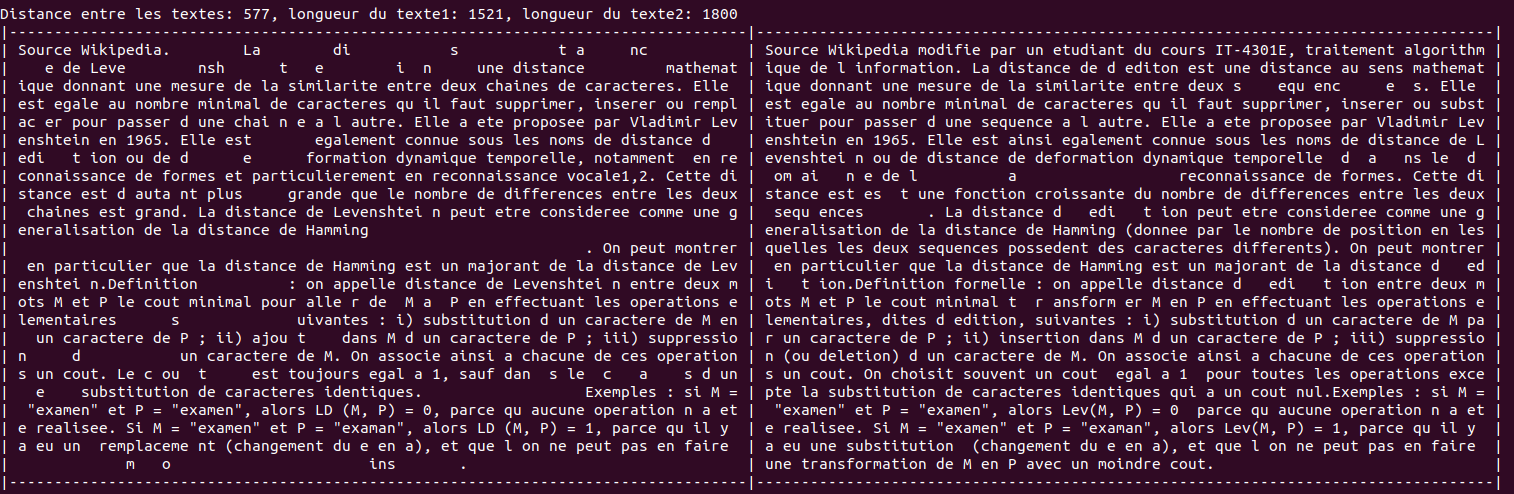
\includegraphics[width=0.95\linewidth]{./images/exo3.png}
	\caption{Résultat de l'alignement des textes}%
	\label{fig:exo3}
\end{figure}
%==============================================================================
\section{Exercice 4}
\subsection{Théorie}
\subsubsection{Algorithme}
Le principal changement ici est que nous voulons mettre en correspondance des
lignes entre elles (séparées par des \textbackslash{}n).\\
Précédemment nous alignions un texte composé de caractères, mais maintenant nous
voulons aligner un texte composé de lignes/phrases/paragraphes qui seront nos
éléments de "base".\\

Le problème étant très similaire au précédent, la méthode que nous utilisions
devrait pouvoir être adaptée à ce nouveau problème.\\
Pour ce faire nous allons définir une nouvelle distance de Levenshtein agissant sur
des lignes entières et plus uniquement des caractères.
Nous allons définir la substitution, insertion, et suppression comme suit:

\begin{gather*}
	\text{Ins'}(y) = Lev(\epsilon,y) = \lvert y \rvert\\
	\text{Del'}(x) = Lev(x,\epsilon) = \lvert x \rvert\\
	\text{Sub'}(x,y) = Lev(x,y)
\end{gather*}
Ici Lev(x,y) est la distance de levenshtein définie précédemment, et x et y
sont des lignes.\\

Il est assez facile de voir pourquoi nous avons choisi comme coût d'insertion
et de suppression la longueur du paragraphe. En effet cela correspond à ajouter
(resp. enlever) les caractères un par un, avec un coût de 1 à chaque fois.\\

Pour la substitution il est un peu moins clair au premier abord sur quelle
valeur choisir. Le choix le plus simple est de supprimer puis d'insérer les
paragraphes, cependant ce ne serait pas une distance car dans ce cas là
$Sub(x,x) \neq 0$.\\
Nous avons étudié plusieurs distances entre les textes, chacunes avec leur
défauts et avantages, mais celle qui paraît la meilleure est la distance de
Levenshtein, qui nous donnera une meilleure indication de la différence entre
nos paragraphes, et nous permettra ensuite facilement de créer un alignement
ayant du sens.\\
Puisque nous avons considéré un coût d'ajout et de suppresion d'un caractère de
1 pour définir $Sub'$ et $Ins'$ nous devons faire pareil dans la distance de
Levenshtein, et nous considérerons un coût de substitution de 1 si les
caractères dont différents et 0 sinon.\\

Nous pouvons ensuite définir notre nouvelle distance de Levenshtein comme suit:
\begin{equation*}
	Lev'(x.a,y.b)= min
		\begin{cases}
			Lev'(x.a,y) + Ins'(b)\\
			Lev'(x,y.b) + Del'(a)\\
			Lev'(x,y) + Sub'(a,b)
		\end{cases}
		= min
		\begin{cases}
			Lev'(x.a,y) + \lvert b \rvert\\
			Lev'(x,y.b) + \lvert a \rvert\\
			Lev'(x,y) + Lev(a,b)
		\end{cases}
\end{equation*}
Ici $a$ et $b$ ne sont plus des caractères mais sont désormais des
paragraphes.\\
Nous sommes donc en mesure d'adapter le code précédemment écrit pour cette
nouvelle version, sans faire beaucoup de changements.\\

Nous pouvons nous demander si $Lev'$ est toujours une distance.\\
Étant donné que $Lev$ est une distance et aue $Sub'(x)=Ins'(x)$ nous pouvons
conclure que nous avons bien une distance.\\


Pour l'algorithme de construction de l'alignement optimal, il est identique à
celui vu précédemment, en adaptant juste la reconstruction des paragraphes.\\
Si nous avons choisi $Ins'$ ou $Del'$ nous construisons une chaine de caractère
vide.\\
Si nous avons choisi $Sub'$ nous construsions l'alignement optimal entre nos
deux paragraphes comme nous l'avons fait précédemment.

\subsubsection{Complexité}

L'algorithme va remplir $n \times m$ cases (n et m étant le nombre de
paragraphes des textes que nous souhaitons aligner).\\
Il faut donc trouver la complexité de $Lev'$ afin de conclure sur la complexité
totale.\\
Les complexités des différentes opérations sont:
\begin{itemize}
	\item $Lev'(x.a,y) + \lvert b \rvert$ a une complexité en $O(\lvert b
		\rvert)$ dans le pire des cas (comme \textit{strlen} en C) 
	\item $Lev'(x,y.b) + \lvert a \rvert$ a une complexité en $O(\lvert a
		\rvert)$ dans le pire des cas (comme \textit{strlen} en C) 
	\item $Lev'(x,y) + Lev(a,b)$ a une complexité en $O( \lvert a \rvert \times
		\lvert b \rvert)$
\end{itemize}

Si nous notons $l$ la longueur du plus long paragraphe, la complexité de calcul
de $Lev'$ est alors $O(l^2+l+l) = O(l^2)$.\\
La complexité totale du calcul de la table est donc $O(m \times n \times l^2)$.\\

Nous avons vu la complexité pour calculer la table des ditances, regardons
maintenant pour la construction de l' alignement optimal.\\
Pour aligner deux paragraphes, si nous avons gardé en mémoire les tables des
distances de Levenshtein utilisées pour le calcul de $Sub'$ lors de la
construction de la table de $Lev'$ la complexité sera de $O(l)$.\\
Si en revanche nous ne les avons pas gardé en mémoire (comme dans notre
implémentation) la complexité sera alors de $O(l^2)$ pour reconstruire la table
puis $O(l)$ pour construire l' alignement dans le cas où l' opération choisie
est la substitution. Dans ce cas, la complexité de la construction de
l'alignement de deux paragraphes est $O(l^2)$ si nous avons choisi la
substitution et $O(l)$ sinon. Il serait alors intéressant en cas d'égalité de
choisir l'opération la moins coûteuse.

Nous obtenons alors une complexité totale pour la construction de l'alignement 
des textes de $O((m+n)\times l^2)$ si nous n'avons pas gardé les tables en
mémoire et et de $O((m+n)\times l)$ si nous l'avons fait.


\subsection{Implémentation}

L'implémentation pour le calcul de la table est presque identique à celle de
l'exercice 3, nous avons juste changé le calcul de sub, ins et del.\\
Le code est disponible en annexe des lignes 324 à 373.\\
Afin de séparer les différents paragraphes des textes, nous avons implémenté
une fonction utilisant \textit{strtok\_r} qui devrait donc être compatible sur tous les
OS, qu'ils respectent les normes POSIX ou non.\\
Son implémentation est fournie en annexe aux lignes 307 à 322.\\

Pour le backtracking aussi le principe reste le même.\\
Pour l'alignement si nous avons fait une insertion ou suppression nous allons
implement insérer une chaîne remplie du caractère vide de bonne longueur.\\
Si nous avons fait une substitution nous allons alors insérer l'alignement
entre les deux textes substitués.\\
Le code est disponible en annexe des lignes 375 à 439.\\

\begin{figure}[!hbt]
	\centering
	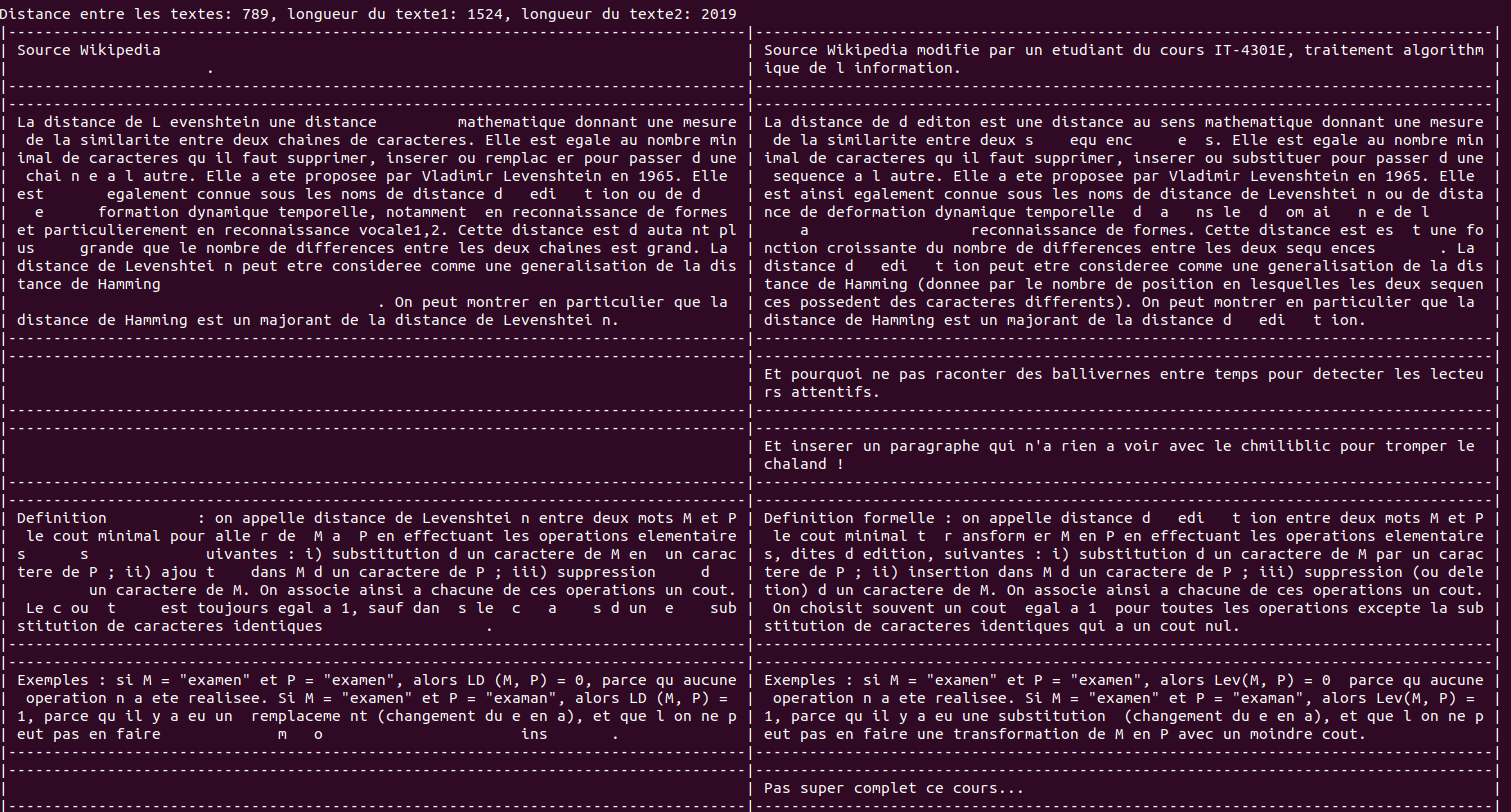
\includegraphics[width=0.95\linewidth]{./images/exo4.png}
	\caption{Résultat de l'alignement des textes paragraphe par paragraphe}%
	\label{fig:exo4}
\end{figure}

Comme nous pouvons le voir sur la figure~\ref{fig:exo4}, nous obtenons bien un
bon alignement des deux textes, identique au résultat attendu, à quelques
détails d'affichage près.\\

D'après les tests et vérifications que nous avons effectuées avec Valgrind, le
programme ne comporte aucune fuite mémoire.\\


\clearpage
%=============================================================================
\section{Annexe: Code source}
		\lstinputlisting[label=code,style=CStyle]{../TD2.c}

\end{document}
